\documentclass[11pt]{article}
\usepackage{style/aaai}
\usepackage{times}
\usepackage{url}
\usepackage{latexsym}
\usepackage{color}
\usepackage{bm}
\usepackage{graphicx}
\usepackage{amsmath}
\usepackage{xspace}
\usepackage{multirow}
\usepackage{subfigure}
\usepackage{bbm}
\usepackage{threeparttable}

% new commands for editing
\newcommand{\prob}[2]{\Pr \left( #1 \,|\, #2 \right)}
\newcommand{\mult}[2]{\mathrm{Mult} \left( #1 \,|\, #2 \right)}
\newcommand{\dir}[2]{\mathrm{Dir} \left( #1 \,|\, #2 \right)}
\newcommand{\tabincell}[2]{\begin{tabular}{@{}#1@{}}#2\end{tabular}}
\newcommand{\newcite}[1]{\citeauthor{#1}~\shortcite{#1}}

% commands for text colors
\newcommand{\red}[1]{{\color{red}{#1}}}
\newcommand{\blue}[1]{{\color{blue}{#1}}}
\newcommand{\green}[1]{{\color{green}{#1}}}
\newcommand{\magenta}[1]{{\color{magenta}{#1}}}

% commands for terms
\newcommand{\stlda}{ST-LDA\xspace}
\newcommand{\stlouis}{St.~Louis\xspace}
\newcommand{\obamatalk}{\emph{Obama Talk}\xspace}
\newcommand{\protest}{\emph{Protest}\xspace}
\newcommand{\racism}{\emph{Racism}\xspace}
\newcommand{\curfew}{\emph{Curfew}\xspace}
\newcommand{\michaelbrown}{\emph{Michael Brown}\xspace}
\newcommand{\newsreport}{\emph{News Report}\xspace}
\newcommand{\pray}{\emph{Pray}\xspace}
\newcommand{\shootincident}{\emph{Shoot Incident}\xspace}
\newcommand{\emotion}{\emph{Emotion}\xspace}
\newcommand{\raceandcommunity}{\emph{Race and Community}\xspace}

% commands for comments
%\newcommand{\psrcomment}[1]{\textcolor{green}{[PSR: {\bf #1}]} }
%\newcommand{\wycomment}[1]{\textcolor{blue}{[WY: {\bf #1}]} }
%\newcommand{\lhcomment}[1]{\textcolor{magenta}{[LH: {\bf #1}]} }
%\newcommand{\vfmcomment}[1]{\textcolor{red}{[VFM: {\bf #1}]} }

%Use these comment definitions to see paper without comments
\newcommand{\psrcomment}[1]{}
\newcommand{\wycomment}[1]{}
\newcommand{\lhcomment}[1]{}
\newcommand{\vfmcomment}[1]{}

%\setlength\titlebox{5cm}
\nocopyright

\title{Uncovering Topic Dynamics of Social Media and News: the Case of Ferguson}

\author{}
%\author{Lingzi Hong \\
%  iSchool \\
%  University of Maryland \\
%  College Park, MD \\
%  {\tt lzhong@umd.edu} \\\And
%  Weiwei Yang \\
%  Computer Science \\
%  University of Maryland \\
%  College Park, MD \\
%  {\tt wwyang@cs.umd.edu} \\\And
%  Philip Resnik \\
%  Linguistics and UMIACS \\
%  University of Maryland \\
%  College Park, MD \\
%  {\tt resnik@umd.edu} \\\And
%  Vanessa Frias-Martinez \\
%  iSchool \\
%  University of Maryland \\
%  College Park, MD \\
%  {\tt vfrias@umd.edu }\\
%}

\date{}

\begin{document}

\maketitle

\begin{abstract}
Looking at the interactions between news content and social media content can help us to understand the increasingly complex dynamics of the relationship between the media and the public surrounding noteworthy news events. Although topic models such as Latent Dirichlet Allocation (LDA) are a valuable tool, they are a poor fit for analyses in which some documents, like news articles, tend to incorporate multiple topics, while others, like tweets, tend to be focused on just one. In this paper, we propose a new model, Single Topic LDA (\stlda), which jointly models news-type documents as distributions of topics and tweets as having a single topic; the model improves topic discovery in news and tweets within a unified topic space by removing noisy topics that conventional LDA tends to assign to tweets in a mixed collection of documents. Using \stlda, we focus on the unrest in Ferguson, Missouri after the fatal shooting of Michael Brown on August 9, 2014, looking in particular at the topic dynamics of tweets in and out of \stlouis area, and at differences and relationships between topic coverage in news and tweets.
\end{abstract}


\section{Introduction}
\label{sec:intro}

Cascading activation model is a widely accepted model, which explores the relationship between government, media and the public~\cite{entman1993framing}. The model helps to explain how frame of information extends down from the White House to elites, media and then to the public of the system. It proposes that moving downward along the cascade is easy, while spreading ideas from lower levels to upper requires extra energy because of the strength of power, the independent environment for decision and comprehensiveness. As the cascade goes down with framing of work from upper layers, the information becomes limited to highlights. The model assumes a certain direction of information flow. Although it acknowledges variation and the possible ways that news feeds back information about the public to influence actions of higher levels, the stair structure emphasizes heavily on the influence from media to the public. However the emergence of social networks makes us think that the situation has changed. 

The creation of social networks aims to provide everyone with equal access to the world, to encourage more independent role in expression, and to achieve information democracy. It has led to increasing participation of information spread, opinion expression and activism by providing easier information access to diverse roles~\cite{kelly2006protest,gonzalez2011dynamics,tufekci2012social}. Social networks become a new competition battlefield for different frames, because everyone can share, comment and create any information. Broader penetration of certain frames becomes more difficult. Politicians even utilize astroturfing, smear campaigns to influence users' choices~\cite{ratkiewicz2010detecting}. On the other side, influence that comes from the public may gain power because they are able to participate and even organize activities online. During the Arab Spring, Twitter has promoted the protest mobilization through reporting real-time event and provided basis for collaboration and emotional mobilization~\cite{breuer2014social}.

It leads us to rethink about the cascade model, specifically on the blurring role of media and users. As a special function role in society, media is still distinctive, but information spreading between media and the public is in both directions, so we want to study whether the power of influence is blurred for media and the public. The following two questions are emphasized:

\begin{enumerate}
\item Is the public still heavily influenced by frames of the media?
\item Does the media pay attention to what the public concerns and reflect the voice from the public?
\end{enumerate}

The influence is hard to detect, considering the difficulty of capturing the status of the public before and after media news. However, we can study the topics of users and media and how these topics are related in time series, as an evidence of media coverage of the public opinions, or influence of media on users.  

In this study, we take Ferguson unrest event in 2014 as an example, to analyze news and tweets topics along with the evolvement of the case. Based on latent Dirichlet allocation~\cite[LDA]{blei2003latent}, Single Topic LDA (\stlda) is proposed to bring long news documents and short tweets under a unified topic frame, so that topics of news and tweets are comparable. From intuition, we assume that long news documents are comprised with multiple topics, while each tweet has only one topic because of the length limitation. Then daily distribution of topics of news and tweets are compared. We also analyze the difference of topics in geography, hypothesizing that geographical culture congruency may lead to different focuses of the public and thus various reactions to media topics.

The contribution of this study lays in three main aspects. First, we tackle the technical problem of building topic model for a mixture of short and long documents. Conventional topic models such as LDA and PLSA~\cite{hofmann1999probabilistic} perform badly on because co-occurrence patterns in short texts are sparse. Consider a tweet with 5 words, every word's topic assignment makes up 20\% of its topic proportion, but usually a tweet's main topic is decided by 2 or 3 words. In this case, the main topic proportion is about 40\% to 60\%, which does not reflect the truth. Our model considers the words in a tweet as a whole and assigns only one topic to a tweet, so that the main topic is more likely to be assigned.
Second, this preliminary study offers a method to understand which are strong frames, which has been a challenge for social scientists~\cite{chong2007framing}. By examining the topic dynamics between news and social media, which are separately representative of media and the public, we may understand which news is influential or which frames are more competitive by analyzing opinions of the public.
Third, bringing tweets and news to the same topic frames will help us to understand large volumes of tweets through news, thus in a more understandable way. When training topic models separately on news and tweets, it is not easy to understand how topics in news and tweets match each other. When combining tweets and news together for analysis, on the other hand, the latent meaning of a topic is the same for tweets and news. Thus large amount of tweets can be represented by news with similar topic distribution, which makes it easier to know public opinions and estimate for opinion poll. 


\section{Related Work}
\label{sec:related_work}

We aim to study the interaction between media and the public by studying dynamics of news and tweets topics during the Ferguson unrest event. The most related research topics are agenda setting online. Political social scientists have noticed the change brought by Internet.~\newcite{sayre2010agenda} propose the question of roles and agenda setting form in the digital age. They manually analyze thousands of videos and news media on Proposition 8 in California, and find that post content in open social media reflects mainstream news, while posts also have influence on professional media coverage, thus create opinion dynamics. The results innovatively reveal the relationship between media and the public in a descriptive way. However it needs large amount of human efforts to apply this method to other events, and it is hard to identify the weight change of topics during the evolving process.

Topic detection has been widely studied for news and social media. Tracking of memes on the Internet is a way to understand dissemination of certain information content. Memes are entities that represent units of information at the desired level of detail~\cite{ratkiewicz2010detecting}. The semantic units play as clear clues for detecting dynamic change of diverse topics.~\newcite{leskovec2009meme} introduce a meme-tracking technique and use it to track topic shifts in news and blogs over a long time. They observe a 2.5-hour lag between peaks of attention to a phrase in the news media and in blogs, which shows evidence of possible interaction between media and other individuals. It involves tracking of repeating semantic entities, as a way for topic tracking, but according to the algorithm only repeated topics, thus memes, can be detected. Entity extraction is also a way to track information diffusion on the Internet.~\newcite{kim2012event} extract 5W1H (\emph{Who}, \emph{What}, \emph{Where}, \emph{When}, \emph{Why} and \emph{How}) structure from events and detect the connection between news, blogs and social networking in a supervised way. However entity expression is limited to specific events rather than topics or frames.

As a big collection of crowding sourcing opinions, tweets have been studied a lot to understand public opinions in social events such as the 2011 Tunisian and Egyptian Revolutions~\cite{gonzalez2011dynamics}, information sharing in protest during the G20 meetings in 2009~\cite{earl2013protest}, and organization of movement in the Occupy Wall Street protest~\cite{conover2013geospatial}. These studies focus more on information flow between different roles rather than the evolving of topics. Topic detection in tweets has been studied because there is challenge for the short length of texts~\cite{yan2013biterm,zhao2011comparing}.

Aggregating short tweets into long document units is a way to alleviate the problem, such as author-based aggregation which is used to identify user topics and measure user similarity~\cite{weng2010twitterrank}. Aggregation based on time slices is used to track emerging events in Twitter~\cite{lau2012line}.~\newcite{hong2010empirical} also propose a method to aggregate tweets by similar words, which tend to work better than regular LDA. However the performance of these methods depends much on the research question and available datasets.

Other variations of topic model are proposed to discover topics from tweets. Biterm topic model~\cite[BTM]{yan2013biterm} directly simulates the generation of word co-occurrence patterns in corpus, thus enhances learning and leads to more coherent topics. A similar model is Word Network Topic Model~\cite{zuo2014word}, which also utilizes word co-occurrence network to solve the sparsity problem.~\newcite{zhao2011comparing} propose a Twitter-LDA model, which assumes that a single tweet is usually about a single topic, to discover topics from a representative sample of the entire Twitter. Supervised methods have also been applied to find tweets topics, such as Labeled-LDA~\cite{ramage2009labeled}, which maps the content of the tweets into dimensions of substance, style, status and social characteristics~\cite{ramage2010characterizing}.

There are studies working on alignment of events information and tweets, which are similar to our work.~\newcite{hu2012lda} propose a joint Bayesian model for events transcripts and tweets, which supposes that event information can impost topical influence on tweets.~\newcite{gao2012joint} create a joint topic model to extract important and complementary pieces of information across news and tweets, and generate complimentary information from both. These models infer tweets topics incorporating information from event transcripts or news. So tweets and event or news topics are under a unified frame. The difference is that, in our method, each tweet is treated to have one topic instead of a probability of distribution of topics. We bring news and tweets together for training, and prove that \stlda model performs better for discovery of topic dynamics.


\section{Method}
\label{sec:model}

\subsection{Dataset}
\label{subsec:dat}
We collected 13,238,863 tweets from August 10, 2014 to August 27, 2014 mentioning Ferguson using the Twitter Streaming API. Among them 92,184 are geo-tagged, which takes about 0.70\% of all. We use geo-tagged tweets instead of all tweets so that we could separate tweets in \stlouis from those are not. We use 2014 TIGER/Lines Shapefile to identify the locations of tweets according to coordinates.\footnote{\url{https://www.census.gov/geo/maps-data/data/tiger-line.html}}

News are crawled by the links published by news account on Twitter. We selected 108 media accounts from Twitter, for example ``Washington Post", ``NBC News" and ``ABC7News", collected all the tweets they published during the Ferguson event, and extracted news reports from the links they published. In total, there are 1,338 news covering from August 11 to 27.

Same standard preprocessing procedure is applied to news and Twitter corpora, such as tokenization, POS tagging, lemmatization, bigrams detection, stop words, low frequency words and too high frequency words removal. After preprocessing and removing empty documents, there are 1,275 news documents and 81,553 Twitter documents, as well as a vocabulary with 1,132 words.

%However, we use different tools for the two corpora: OpenNLP package~\cite{baldridge2005opennlp} for news corpus and Tweet NLP package~\cite{owoputi2013improved} for Twitter corpus.

\subsection{Single Topic LDA Model}

We propose \stlda to deal with short documents like tweets and long documents like news simultaneously. The intuition is that short documents are unlikely to be related to multiple topics. Instead, one short document is usually talking about a single topic and all its words are generated from this topic. Meanwhile, long documents still follow conventional LDA assumptions: each document contains a mixture of topics. Specifically, the generative process of tweets and news is defined as

\begin{enumerate}
\item For each topic $k \in \{1, \ldots, K\}$
    \begin{enumerate}
    \item Draw word distribution $\bm{\phi_k} \sim \mathrm{Dir}(\beta)$
    \end{enumerate}
\item For each news document $d\in \{1, \ldots, D^\mathrm{N}\}$
    \begin{enumerate}
    \item Draw topic distribution $\bm{\theta^{\mathrm{N}}_{d}} \sim \mathrm{Dir}(\alpha)$
    \item For each token $t^{\mathrm{N}}_{d,n}$ in news document $d$
        \begin{enumerate}
        \item Draw a topic $z^{\mathrm{N}}_{d,n} \sim \mathrm{Mult}(\bm{\theta^\mathrm{N}_d})$
        \item Draw a word $w^{\mathrm{N}}_{d,n} \sim \mathrm{Mult}(\bm{\phi_{z^{\mathrm{N}}_{d,n}}})$
        \end{enumerate}
    \end{enumerate}
\item Draw tweet background topic distribution $\bm{\theta^{\mathrm{T}}} \sim \mathrm{Dir}(\alpha)$
\item For each tweet document $d \in \{1, \ldots, D^\mathrm{T}\}$
    \begin{enumerate}
    \item Draw a topic $z^{\mathrm{T}}_d \sim \mathrm{Mult}(\bm{\theta^{\mathrm{T}}})$
    \item For each token $t^{\mathrm{T}}_{d,n}$ in document $d$
        \begin{enumerate}
        \item Draw a word $w^{\mathrm{T}}_{d,n} \sim \mathrm{Mult}(\bm{\phi_{z^{\mathrm{T}}_d}})$
        \end{enumerate}
    \end{enumerate}
\end{enumerate}

The corresponding graphical model is given in Figure~\ref{fig:stlda}.

\begin{figure}[h]
\centering
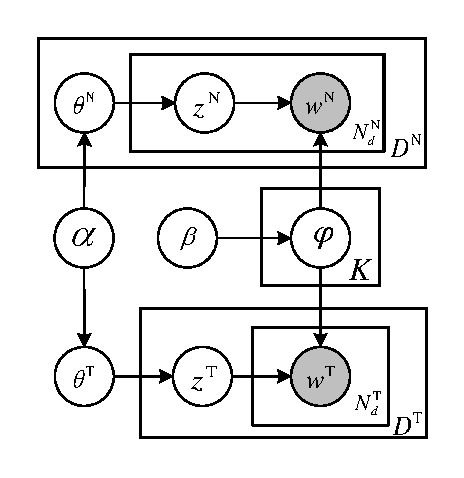
\includegraphics[width=.8\linewidth]{figures/stlda_model.pdf}
\caption{Graphical Model of \stlda}\label{fig:stlda}
\end{figure}

The model's news part is the same as that of conventional LDA, but its tweet part is different. Specifically, the coverage of two plates are different, which is adapted according to our assumptions. The first difference is the coverage of word plate (the one with subscript $N^\mathrm{T}_d$). In LDA, it covers both $\bm{z}$ and $\bm{w}$, denoting that every word has its own topic assignment and every document consists of a mixture of topics. In \stlda's tweet part, the plate only covers $\bm{w}$, which means that every word in a tweet is generated from the same topic.

The second difference is the coverage of document plate (the one with subscript $D^\mathrm{T}$). LDA assumes that every document has a topic distribution, but in \stlda, every tweet only has one topic which can not form a distribution inside a document. Thus, $\bm{\theta^\mathrm{T}}$ is outside the document plate and denotes a background topic distribution of tweets. The posterior inference of \stlda is done by Gibbs sampling.

%\subsection{Posterior Inference}


%The sampling equation for news documents is the same as conventional LDA. The probability of $n$-th token in news document $d$ being assigned to a topic $k$ is computed as

%\begin{align}
%&\prob {z_{d,n}=k} {\bm{z_{-d}},\bm{w_{-d,n}},w_{d,n}=v} \notag\\
%\propto &\left( N_{d,k}^{-d,n} + \alpha \right) \frac {N_{k,v}^{-d,n} + \beta } {N_{k,\cdot}^{-d} + V\beta},
%\end{align}
%where $N_{d,k}$ denotes the number of tokens in document $d$ assigned to topic $k$; $N_{k,v}$ denotes the count of word $v$ assigned to topic $k$. Marginal counts are denoted by $\cdot$. $^{-d,n}$ denotes that the count excludes the $n$-th token in document $d$.

%The probability of tweet $d$ being assigned a topic $k$ is computed as

%\begin{align}
%&\prob {z_d=k} {\bm{z_{-d}},\bm{w}} \notag\\
%\propto &\left( N_k^{-d} + \alpha \right) \frac {\prod\limits_{v=1}^{V} \prod\limits_{i=0}^{N_{d,v}-1} \left( N_{k,v}^{-d} + \beta + i \right)} {\prod\limits_{i=0}^{N_{d,\cdot}-1} \left( N_{k,\cdot}^{-d} + V\beta + i \right)},
%\end{align}
%where $N_k$ denotes the number of documents assigned to topic $k$; $N_{d,v}$ is the count of word $v$ in document $d$. $^{-d}$ denotes that the count excludes document $d$.

%A brief derivation of Gibbs sampling equation is attached in %Appendix~\ref{sec:derivation}.

% After we train a model on training corpus, we can apply it on unseen documents and infer their topic assignments. The Gibbs sampling equation for test is much simpler. The probability of assigning topic $k$ to document $d$ is

% \begin{equation}
% \prob {z_d=k} {\bm{z_{-d}},\bm{w_d}} \propto \left( N_k^{-d} + \alpha \right) \prod_{v=1}^{V} \phi_{k,v}^{N_{d,v}}.
% \end{equation}

\subsection{Topic Dynamics}
The output results of \stlda model can be used for further discovery of topic dynamics of tweets and news. We define topic dynamics as temporal change of topics using daily sliding window. Assuming that every news document has the same impact and contributes equally to the total media environment, the topic proportion of day $t$ is the average of topic probabilities of all news documents on that day as

\begin{equation}
\bar{\theta}_{t,k}^{\mathrm{news}}=\frac{\sum_{d=1}^{D_t^{\mathrm{news}}} \theta_{d,k}}{D_t^{\mathrm{news}}},
\end{equation}
where $D_t^{\mathrm{news}}$ denotes the number of news documents on day $t$; $\theta_{d,k}$ is topic $k$'s proportion in document $d$.

Differently, each tweet $d$ has only one topic $z_d$ given by \stlda. Under the same assumption that each tweet contributes equally to the voice of public, the aggregation of daily tweet topic proportion is calculated as

\begin{equation}
\bar{\theta}_{t,k}^{\mathrm{tweets}} = \frac{\sum_{d=1}^{D_t^{\mathrm{tweets}}} \mathbbm{1}(z_d=k)}{D_t^{\mathrm{tweets}}},
\end{equation}
where $D_t^{\mathrm{tweets}}$ denotes the number of tweet documents on day $t$ and $\mathbbm{1}(\cdot)$ is an indicator function.

Given $\bm{\bar{\theta}_t^{\mathrm{news}}}$ and $\bm{\bar{\theta}_t^{\mathrm{tweets}}}$ where $t$ varies from August 11 to 27, we can identify topic dynamics by the changing of daily topic proportions. 

\section{Evaluation of Topic Quality}
\label{sec:eva}

Accurate identification of tweet topic is important for analysis of topic dynamics because each tweet performs as a unit to form the component of topics a day. If every tweet is assigned with noisy topics, the significance of main topic will decrease while weight of minor topics may increase. Different from conventional LDA, because of the limitation of tweet length, we assign only one topic for each tweet in the \stlda model. Meanwhile we train news and tweets together so that topics of news and tweets are comparable. In this section, we compare topic quality by LDA and \stlda to prove that \stlda gives reasonable good results and performs better than LDA for analysis of topic dynamics. The hyperparameters $\alpha$ and $\beta$ are both set to 0.1 and the number of topics is set to 10. As topics given by the two models are in different orders, we match topics based on KL divergence before comparing them. The matching procedure starts by obtaining a KL divergence table $T$. Each cell $T_{k_1,k_2}$ stores the KL divergence of topic $k_1$ given by LDA and topic $k_2$ given by \stlda as

\begin{eqnarray}
T_{k_1,k_2}&=&\mathrm{KL}(\bm{\phi_{k_1}^\mathrm{LDA}}||\bm{\phi_{k_2}^\mathrm{\stlda}})\\
&=&\sum_{v=1}^{V} \phi_{k_1,v}^{\mathrm{LDA}} \log_2 \frac{\phi_{k_1,v}^{\mathrm{LDA}}}{\phi_{k_2,v}^{\mathrm{\stlda}}}.
\end{eqnarray}

Then we run a depth-first search algorithm on the KL divergence table to find the best match with smallest overall KL divergence. Meanwhile if one pair has KL divergence larger than a threshold, there is no matching topic.

\subsection{Balanced Topics from Tweets and News}

\begin{table*}[htpb]
\centering
\begin{threeparttable}
\begin{tabular}{|c|c|l|}
\hline
\bf \tabincell{c}{Model\\(Corpus)} & \bf Topic & \multicolumn{1}{c|}{\bf Top Words}\\ \hline
\multirow{5}*{\tabincell{c}{LDA\\(NT)\tnote{1}}} & Obama Talk\tnote{3} & happen, i'm, make, thing, talk, situation, what's, what's\_happen, bad, you're\\ \cline{2-3}
 & Protest & tear\_gas, protester, arrest, fire, medium, rt, protestor, street, crowd\\ \cline{2-3}
 & Racist & black, white, loot, protect, community, racist, stop, race, citizen, riot\\ \cline{2-3}
 & Curfew & missouri, state, obama, national\_guard, call, curfew, mo, press, governor\\ \cline{2-3}
 & Pray & peace, pray, justice, stand, love, tonight, hope, stay, family, safe\\ \hline
\multirow{5}*{\tabincell{c}{\stlda\\(NT)}} & Obama Talk & obama, president, law\_enforcement, house, holder, make, story, post, include\\ \cline{2-3}
 & Protest & tear\_gas, arrest, protester, fire, rt, reporter, medium, shoot, crowd\\ \cline{2-3}
 & Racist & black, white, make, race, america, obama, stop, happen, situation, riot\\ \cline{2-3}
 & Curfew & missouri, curfew, state, national\_guard, governor, nixon, call, gov, order\\ \cline{2-3}
 & Pray & peace, pray, stand, justice, night, love, tonight, today, family\\ \hline
\multirow{5}{*}{\tabincell{c}{LDA\\(N)\tnote{2}}} & Obama Talk & obama, president, house, make, white, news, national, deal, run, defense\\ \cline{2-3}
 & Protest & st\_louis, nixon, protester, shooting, county, justice, aug., investigation, state, thursday\\ \cline{2-3}
 & Racist & black, make, white, cop, time, don't, year, good, man, thing\\ \cline{2-3}
 & Curfew & protester, johnson, tear\_gas, crowd, curfew, night, fire, street, missouri, shoot\\ \cline{2-3}
 & Pray & (No matching topic)\\ \hline
\end{tabular}
\begin{tablenotes}
\footnotesize
\item[1] NT: news and tweets.
\item[2] N: news only.
\item[3] This topic is matching with \obamatalk in \stlda. Although top words show it is about question of the situation, for comparison we still name the topic with \obamatalk.
\end{tablenotes}
\caption{Topic Examples}\label{tab:topic}
\end{threeparttable}
\end{table*}

To make sure that \stlda has balanced topics that come from both tweets and news, we train another model merely on news and set the results as a baseline for comparison. Table~\ref{tab:topic} shows four common topics for all three models and one topic that only exists in results trained on news and tweets together. Four common topics indicate that news topics are kept when mixture of documents are trained together. But there is no matching topic in the baseline results corresponding to the topic \pray in LDA and \stlda on NT, which means \pray tends to only exists in tweets. Meanwhile top words in the four common topics are different. Emergence of Twitter language such as \emph{rt} and \emph{gov} in top words indicate topics from tweets. So \stlda can extract topics from both news and tweets, not biased to one type of texts, and it discovers topics that exist in both news and tweets.

\subsection{Topic Quality for Tweets}
\label{subsec:intrinsic}
%Perplexity is usually employed to quantitatively evaluate the topic quality. It is computed based on every single word. However, \stlda treats each tweet as a whole, not single words, so perplexity is not applicable to evaluate topic quality of LDA and \stlda. Therefore, we evaluate topic quality qualitatively instead of quantitatively.

Accurate topic assignment is important for analysis of topic dynamics. In this part we pick several tweets and evaluate quality of topic assignment by \stlda. We list five tweets in Table~\ref{tab:tweets} and manually labeled with the main topic. Topic assignments by LDA and \stlda are given in Table~\ref{tab:tweet_topic}. Topics in LDA and \stlda are matched and numbered from 0 to 9. Names of topics are manually summarized according to top frequency words in the topic.

\begin{table*}[htpb]
\centering
\begin{tabular}{|c|c|p{13cm}|}
\hline
\bf No. & \bf Label & \multicolumn{1}{c|}{\bf Content}\\ \hline
1 & Protest & ``@bkesling: ``Hands up, don't shoot" after tear gas fired in \#Ferguson http://t.co/9zQIh31wQg" modern day America...  \#PrayForFerguson\\ \hline
2 & Race & 80\% black folks think \#Ferguson raises ``important issues about race that need to be discussed," only 37\% of white folks do. Very sad.\\ \hline
3 & Police & You guys can't blame that cop in \#Ferguson. Shooting your gun 6 times is literally the answer to every question in their training manual.\\ \hline
4 & Protest & \#fergusongate media get it straight. U act like those who don't live in ferguson can't protest. This is for all blacks everywhere.\\ \hline
5 & News & But thank God for social media though. Imagine if we're dependent on the news to tell the ``truth" about what's really happening in \#Ferguson\\ \hline
\end{tabular}
\caption{Tweet Examples}\label{tab:tweets}
\end{table*}

\begin{table*}[htpb]
\centering
\begin{tabular}{|c|c|c|c|c|c|c|c|}
\hline
\multicolumn{3}{|c|}{\bf Tweets} & 1 & 2 & 3 & 4 & 5\\ \hline
\multirow{10}{*}{\tabincell{c}{\bf LDA Topic\\ \bf Distribution}} & 0 & Obama Talk & 0.017 & \bf 0.373 & 0.011 & 0.017 & \bf 0.888\\ \cline{2-8}
 & 1 & Protest & \bf 0.517 & 0.009 & 0.011 & \bf 0.183 & 0.013\\ \cline{2-8}
 & 2 & Racism & 0.017 & \bf 0.555 & \bf 0.233 & 0.017 & 0.013\\ \cline{2-8}
 & 3 & Curfew & 0.017 & 0.009 & 0.011 & 0.017 & 0.013\\ \cline{2-8}
 & 4 & Michael Brown & 0.017 & 0.009 & \bf 0.567 & \bf 0.183 & 0.013\\ \cline{2-8}
 & 5 & News Report & 0.017 & 0.009 & 0.011 & 0.017 & 0.013\\ \cline{2-8}
 & 6 & Pray & 0.017 & 0.009 & 0.011 & 0.017 & 0.013\\ \cline{2-8}
 & 7 & Shoot Incident & \bf 0.350 & 0.009 & 0.011 & 0.017 & 0.013\\ \cline{2-8}
 & 8 & Emotion & 0.017 & 0.009 & \bf 0.122 & \bf 0.183 & 0.013\\ \cline{2-8}
 & 9 & Race and Community & 0.017 & 0.009 & 0.011 & \bf 0.183 & 0.013\\ \hline
\multicolumn{3}{|c|}{\bf \stlda Topic} & 1 & 2 & 4 & 8 & 5\\ \hline
\end{tabular}
\caption{Tweet Topic Comparison}\label{tab:tweet_topic}
\end{table*}

The first tweet is assigned with two topics with relatively high probability by LDA, thus \protest and \shootincident. Although the sentence contains words like \emph{shoot}, it is not appropriate to be assigned with topic 7,which has top words like \emph{street} and \emph{Michael Brown}. Meanwhile the tweet has small probability under other topics such as \obamatalk and \racism, which have nothing to do with the content of the tweet.
Similarly the second tweet mainly talks about racism, which is what \stlda gives, but LDA assignment topic \obamatalk with probability 0.373 and slight probability for other topics. The common pattern is that the topic with highest probability in LDA is consistent with the topic given by \stlda. But case of the fourth and fifth tweets prove that we couldn't just use LDA and assign tweet with the one topic with highest probability.

The fourth tweet is assigned by LDA with 5 topics with equally high probability, thus \protest, \michaelbrown, \shootincident, \emotion and \raceandcommunity. However the tweet doesn't mention Michael Brown incident or shooting things. There are noisy topics in results given by LDA. It assigns part of the probability to wrong topics, which makes the right topic not so significant. This is the shortage of LDA but solved by \stlda. The 5th tweet shows how \stlda assigns the right topic but LDA fails to.

Evaluation of topic quality shows that \stlda has advantage in assigning tweets with one topic, because most of the tweets are short and actually contain only one topic. LDA gives each tweet a probability distribution of topics, which usually contains irrelevant topics and also decreases the importance of right topic. Meanwhile the results of \stlda can't be substituted by assigning the topic with highest probability in the distribution.

%\subsection{Comparison of LDA and \stlda in Topic Dynamics}
%\label{subsec:extrinsic}

%The extrinsic evaluation is conducted to see how the two algorithms perform in showing topic dynamics. We compare the results of topic dynamics in news and tweets. Figure~\ref{fig:news_topics} shows the change of news topic proportions from August 11 to 27 based on the results of LDA and \stlda. It is similar that investigation of shoot accident and discussion of race are the two main themes of news. Along with the evolvement of event, the proportion of race issues increases, while the voice of investigation reaches a peak on August 17 and decreases thereafter.

%\begin{figure*}[htpb]
%\centering
%\subfigure[LDA]
%{
%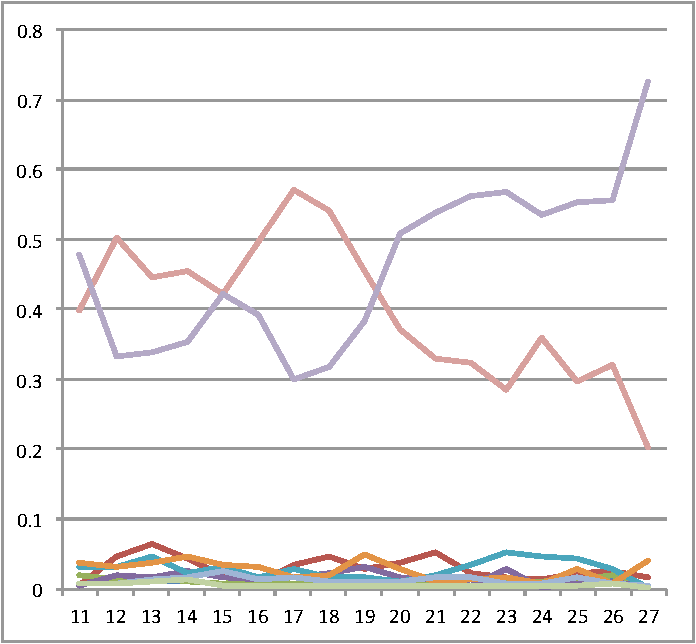
\includegraphics[width=0.48\linewidth]{figures/1LDANews-2.pdf}
%\label{fig:news_topics_lda}
%}
%\subfigure[\stlda]
%{
%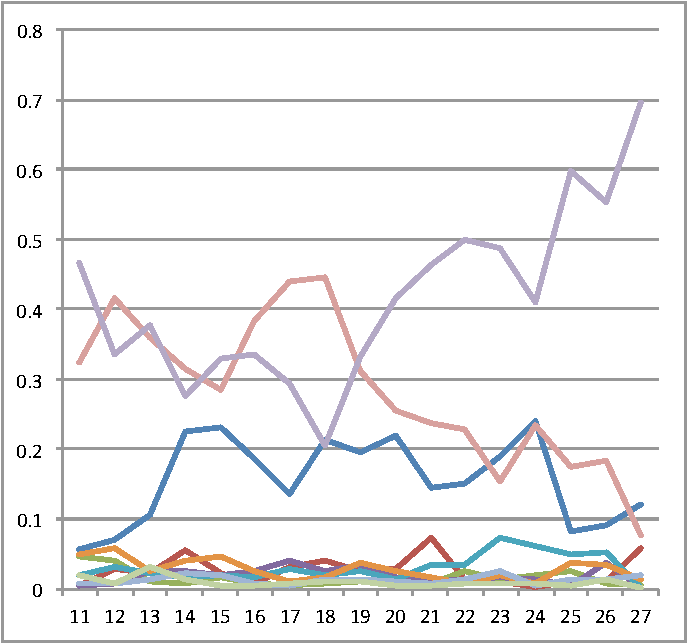
\includegraphics[width=0.48\linewidth]{figures/1STLDANews-2.pdf}
%\label{fig:news_topics_stlda}
%}
%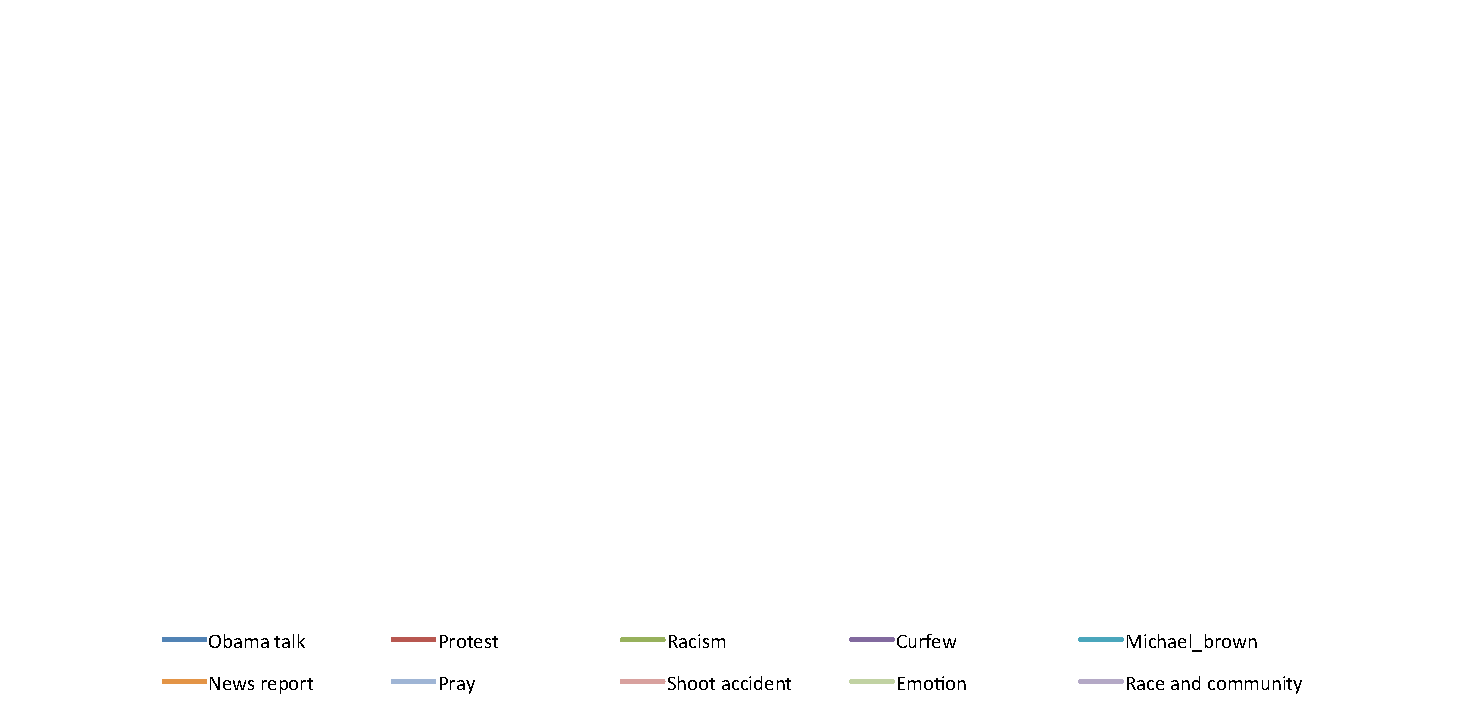
\includegraphics[width=\linewidth]{figures/Legend.pdf}
%\caption{News Topic Dynamics by LDA and \stlda}\label{fig:news_topics}
%\end{figure*}

%Topic distribution given by LDA is highly skewed to two main topics, thus the \shootincident and the \raceandcommunity, while other topics take only a small proportion and it is hard to identify the proportion change of these topics. Meanwhile \stlda gives results that are slightly better in representing different topics. Besides the significant change of \shootincident and \raceandcommunity, the \obamatalk is discovered as a main topic for media. It keeps a relatively stable proportion of 20\%, and peaks after some important events related with Obama. For example, on August 12, Obama addressed the shooting and urged the community in Ferguson to stay calm. On August 14, he gave a talk saying there is no excuse for protesters to turn to violence, which seems to lead to the peak on August 14 and 15. Also in news topic dynamics by \stlda, the \protest shows a peak on August 21, which is consistent with the date when the National Guard withdrew from the Ferguson.

%Both LDA and \stlda are unsupervised methods, so it is hard to verify which topic dynamic reflects the real situation. But the topics discovered by \stlda are more diverse, and are consistent with the important events in the timeline.

%There is more variance in topic dynamics of tweets by \stlda than LDA, which is shown in Figure~\ref{fig:tweets_topics}. The proportion of topics is close to each other in topic dynamics by LDA, so it is relatively hard to identify the main topics for each day. There is rising point of \michaelbrown after the shoot accident, and a peak on August 25 when the funeral for Michael Brown is held. However, consistent with the shortage discussed in analysis of tweet topics, LDA gives a probability distribution of topics, of which some are irrelevant. So when aggregating tweets in a day together, the proportion number for each topic is similar, which makes it hard to identify main topics on that day, and change of topics along the time. Comparatively, \stlda gives results with better representation of topic dynamics. There is variation of topics changing overtime. It is clearly that after the shoot accident, emotion of the public surges to a peak on August 11. After the protest event, another emotion topic appears on August 14. Meanwhile, the proportion of \pray topic keeps relatively stable from August 11 to August 24, and increases a lot on the day when Michael Brown's funeral is held. These tendencies in topic changes can be seen in topic dynamics of tweets by LDA, but these topics are entangled with other topics, making it hard to differentiate from other topics.

%\begin{figure*}[htpb]
%\centering
%\subfigure[LDA]
%{
%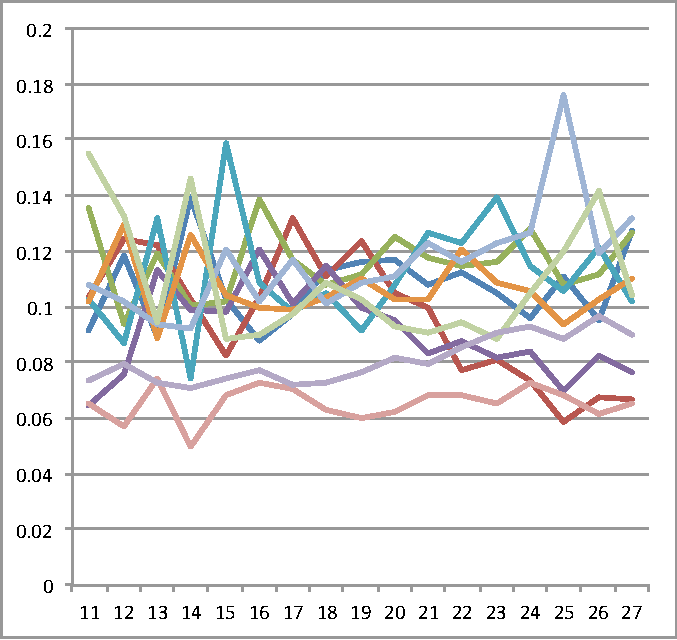
\includegraphics[width=0.48\linewidth]{figures/2LDATweets.pdf}
%\label{fig:tweets_topics_lda}
%}
%\subfigure[\stlda]
%{
%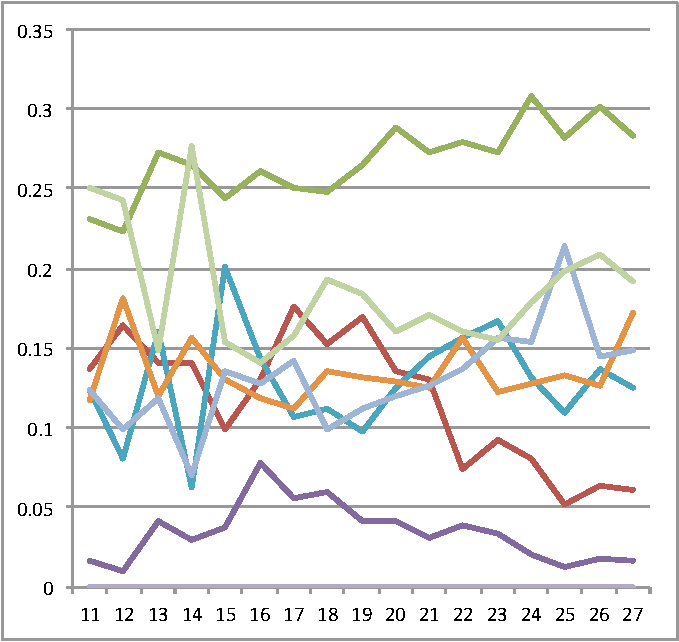
\includegraphics[width=0.48\linewidth]{figures/2STLDATweets.pdf}
%\label{fig:tweets_topics_stlda}
%}
%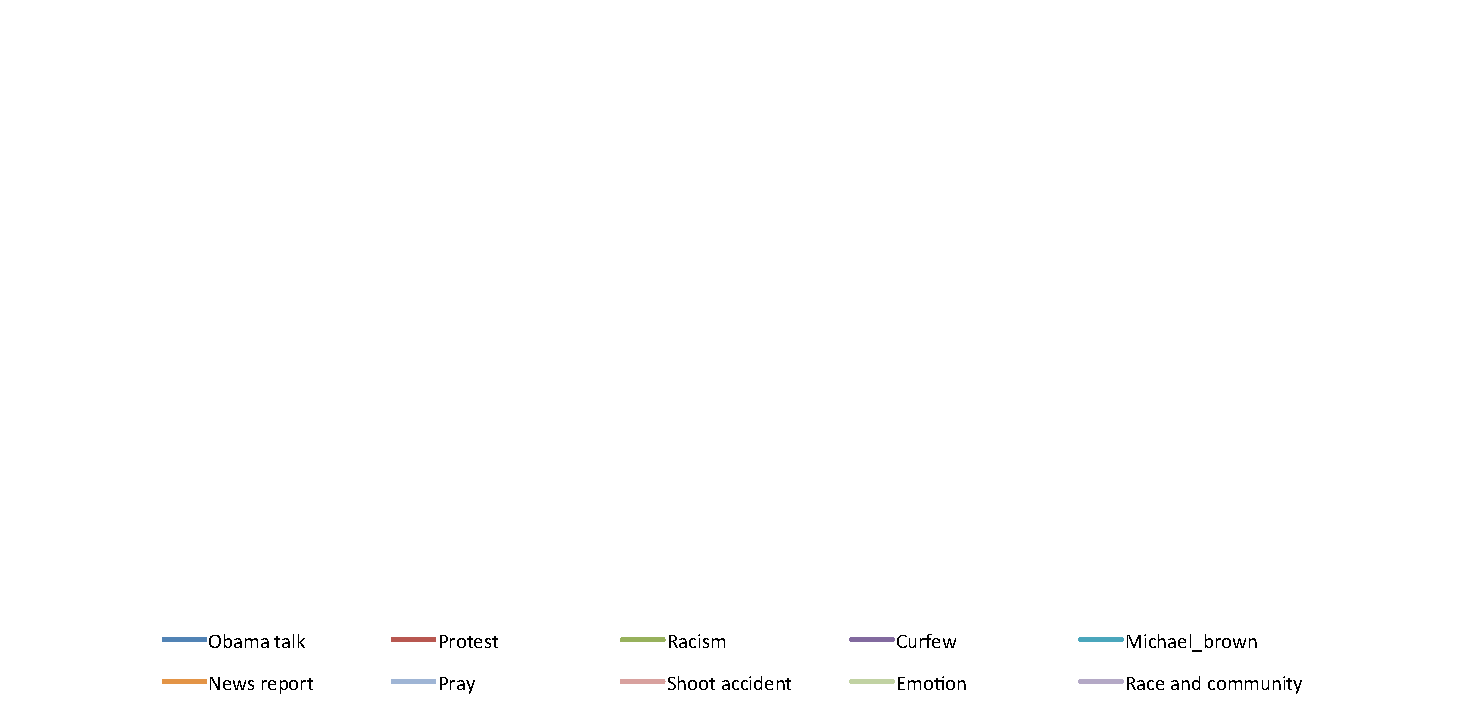
\includegraphics[width=\linewidth]{figures/Legend.pdf}
%\caption{Tweets Topic Dynamics by LDA and \stlda}\label{fig:tweets_topics}
%\end{figure*}

%In summary, by intrinsic and extrinsic evaluation, \stlda is more accurate in assigning one topic to each tweet and giving better results in topic dynamics. %In Section~\ref{subsec:topic_track}, we use the results of \stlda on tweets and news for topic tracking analysis.



\section{Topic Dynamics of Tweets and News}
\label{sec:top}

In this part, we compare topic dynamics of news and tweets based on the results by \stlda. Considering the factor of distance on perception of events~\cite{he2015uncovering}, we analyze topic dynamics for tweets in and out of \stlouis where the Ferguson unrest took place to exclude the influence of geographical difference. To answer the research questions, we compare topics in news and tweets, and how the topic proportion changes everyday. First we related topic dynamics to ground truth events to see the different focus of media and the public, and how news and social media react to real situations. Then we compare topic dynamics of news and tweets in and out of \stlouis area to find out whether there is evidence of influence by media on the public, or shift focus of the media because of topics in tweets.

\begin{figure*}[htpb]
\centering
\subfigure[Tweets in \stlouis]
{
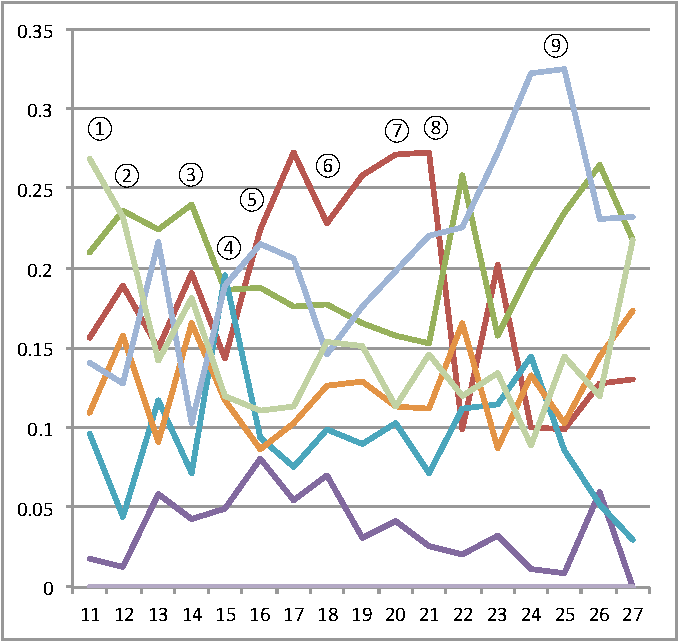
\includegraphics[width=0.32\linewidth]{figures/3LDA2TweetsInSt_revised.pdf}
\label{fig:tweets_topics_inst}
}
\subfigure[Tweets out of \stlouis]
{
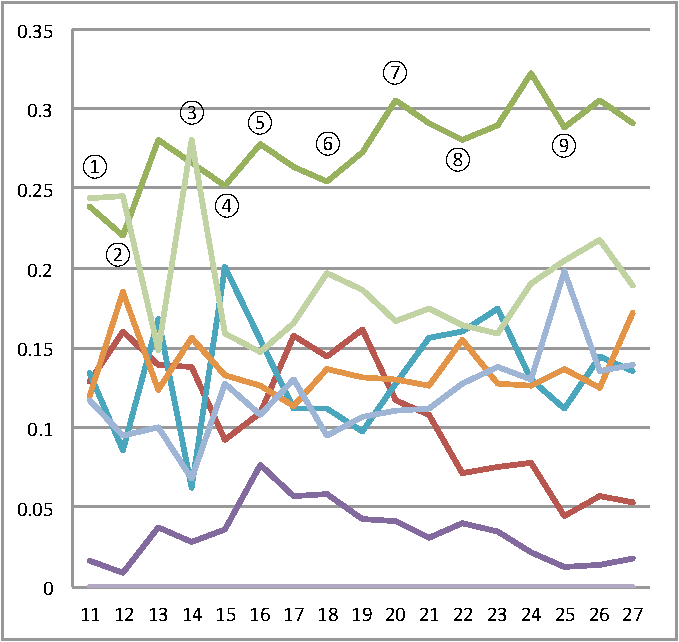
\includegraphics[width=0.32\linewidth]{figures/3LDA2TweetsOutSt_revised.pdf}
\label{fig:tweets_topics_outst}
}
\subfigure[News]
{
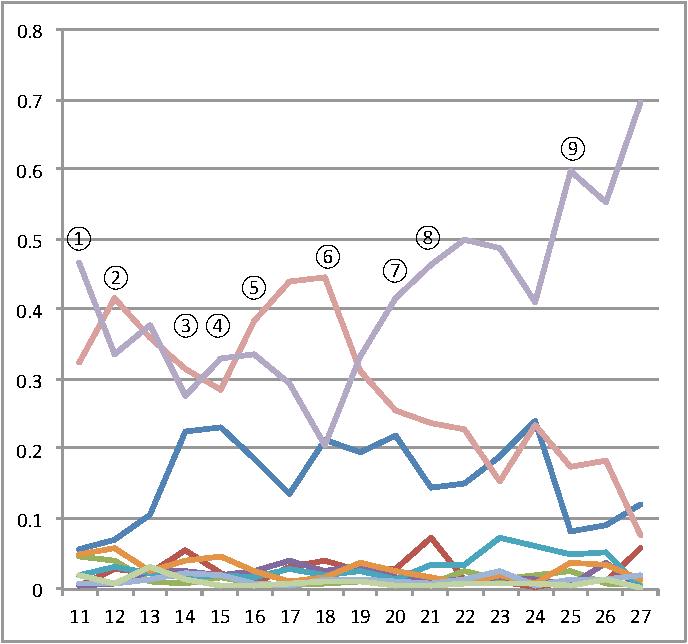
\includegraphics[width=0.32\linewidth]{figures/1STLDANews-2_revised.pdf}
\label{fig:news_topics}
}

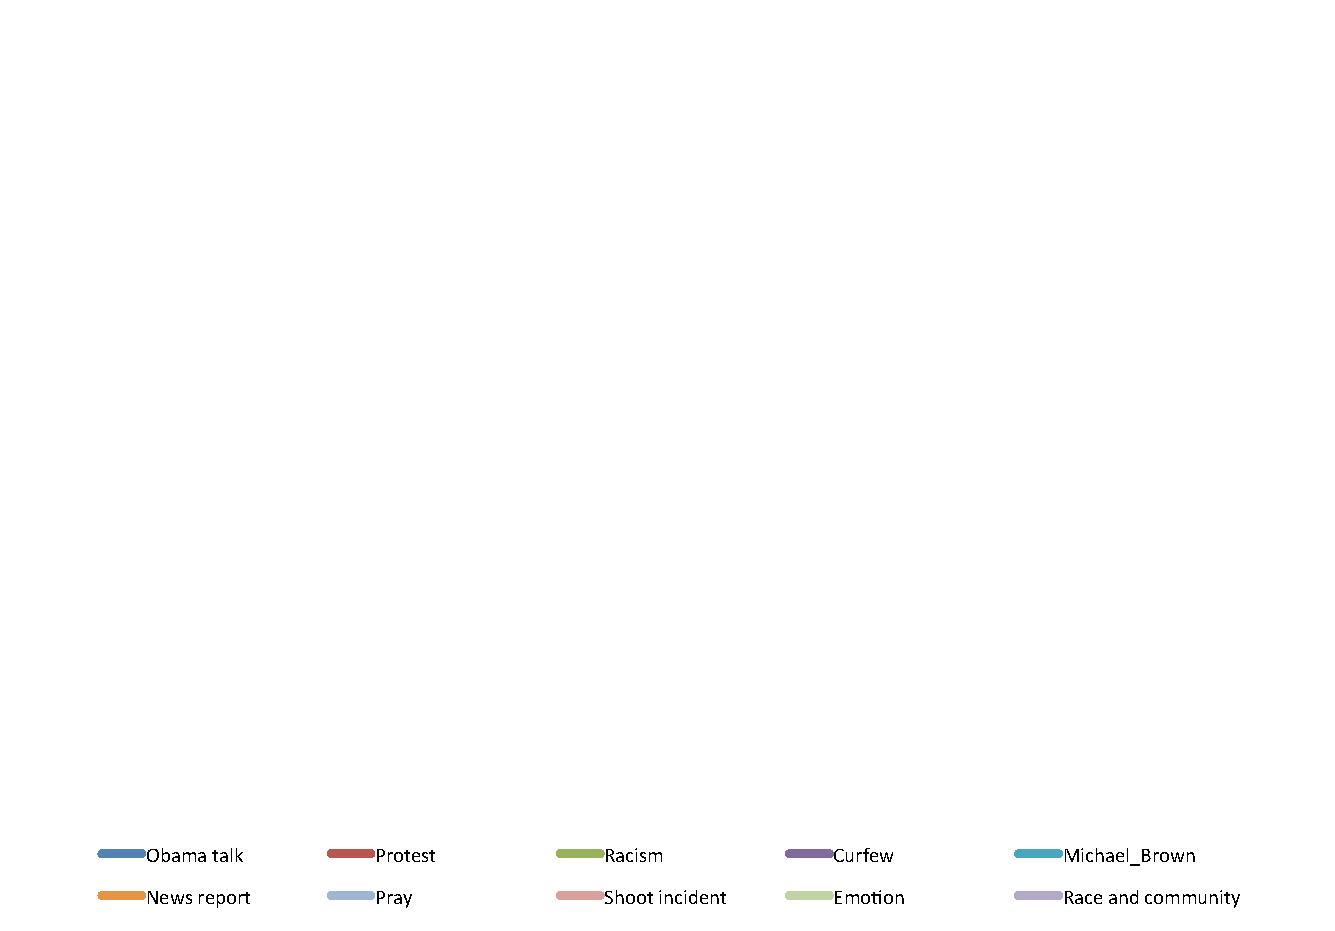
\includegraphics[width=\linewidth]{figures/Legend_revised_cut.pdf}
\caption{Topic Dynamics of Tweets and News by \stlda. Important events: \textcircled{\small{1}} Aug 11: unrest continues; \textcircled{\small{2}} Aug 12: first Obama talk; \textcircled{\small{3}} Aug 14: second Obama talk and Nixon announces law enforcement operation; \textcircled{\small{4}} Aug 15: robbery video is released; \textcircled{\small{5}} Aug 16: curfew is imposed; \textcircled{\small{6}} Aug 18: National Guard is deployed; \textcircled{\small{7}} Aug 20: a grand jury convenes to begin determining of crime and streets become quiet; \textcircled{\small{8}} Aug 21: National Guard withdrew; \textcircled{\small{9}} Aug 25: Michael Brown's funeral.}\label{fig:topic_dynamics}
\end{figure*}

\subsection{Focus Shift Analysis for Tweets and News}
\label{subsec:tweet_topic}
We relate topics of tweets discovered by \stlda with ground truth to analyze focus of the people and how the focus changes along with important events. Ground truth events and the import time points perform as benchmarks. We choose a news report that involves with timeline of important events since Michael Brown's death. Although it is from the view of the media, which have perspectives and may not include all important events, it is a relative complete benchmark with time of shoot incident, looting, FBI investigation, Obama talk, protests, curfew, Michael Brown's funeral and so on.\footnote{\url{http://www.telegraph.co.uk}}

\subsubsection{Tweet Topics in and out of \stlouis Area}
The tweet topic dynamics in and out of \stlouis are shown in Figure~\ref{fig:topic_dynamics}.

Difference in topic dynamics of two sets of tweets show different perception of events for people in and out of \stlouis area. More tweets in \stlouis talk about \protest, while out of \stlouis more tweets talk about \racism. From August 18, when Governor Nixon deployed the National Guard to Ferguson, to August 21 when the National Guard withdrew, protests and conflicts keep occurring. People in Ferguson area are closer and more related to protests, so tweets with this topic surge to take more than 25\% of all tweets. Meanwhile proportion of \protest tweets out of \stlouis is far less. The public not involved in the event tend to have less knowledge about real situations, but according to what they hear and know, they are better at abstract thinking, thus \racism takes majority in most of the time.

An interesting phenomenon is the \emotion topic change. Michael Brown was killed on August 9, and anger emotion is the major topic of tweets in \stlouis, then \emotion tweets keep decreasing, taking 10\% to 15\% of all tweets. However outside \stlouis area, there is a lag effect of \emotion explosion on August 14th. It is possible that news takes time to spread and the public outside Ferguson need more information to understand what happened and brew mood. It is also possible that they are reacting to \obamatalk, which is also a main topic in news.

Topic \curfew, \newsreport and \michaelbrown share similar change patterns for tweets in and out of \stlouis area. \curfew increases to a peak on August 16 when Governor Nixon declared a state of emergency and imposed a curfew. It takes around 5\%, which seems not to be an important issue. Topic \pray shares similar dynamics that there is a large increase of tweets on this topic on August 25 when Michael Brown's funeral is held. More than 35\% of tweets in \stlouis are about \pray, while out of \stlouis is 20\%.

The above topic changes are highly related to ground truth event, however there are evidence that the public could be influenced by media:
\begin{enumerate}
\item Different perception of events: people in \stlouis tend to publish tweets that are more related with evlovement of event such as the shooting, protests and funeral. They behave as witness and reporters. While people out of \stlouis have a lag effect of \emotion explosion and more abstract discussion of \racism. We assume that their knowledge mainly comes from news, social media and other indirect report of the event, so they are more subjected to media influence.
\item Tweets in and out of \stlouis share similar dynamics for topic \newsreport and \michaelbrown. News report is directly about possible media influence. Meanwhile the common peak time of topic \michaelbrown is the day when Police Chief released the video of Brown in robbery before being shot. It is also intuitive that even people in \stlouis perceive such information through outside source such as mass media, as people elsewhere. The similar reaction pattern reflects that they are both possible to be influenced by media in these topics.
\end{enumerate}

\subsubsection{News Topics}
There are three main topic lines in news that are \obamatalk, \shootincident and \raceandcommunity, which do not exist in tweets. According to top words in \shootincident, it is similar to topic \michaelbrown, which takes a certain proportion in tweets, and a few proportion in news. Although news and tweets talk about the same thing, the words they use are quite different, which lead to different topic assignment by \stlda. Similarly, \racism topic exists mostly in tweets, while \raceandcommunity mainly exists in news. Although these two topics are both about race, there is little overlapping of tweets and news in the two topics. One possible reason is that tweets use more oral language, while news uses more formal written language. Another is that media and the public describe the same thing with different frames. According to the top words in two topics, there are more negative words in \racism such as \emph{stop}, \emph{riot}. In the topic labeled with \raceandcommunity, words like \emph{make}, \emph{good}, \emph{community} are indicative of positive emotion. Thus the public tends to have negative emotion about race issues during the Ferguson unrest, but the media tried to describe and lead the discussion to a positive way.

In the main topics, only \obamatalk is related to ground truth events. The proportion of topic \obamatalk increases from August 12 when Obama first address the shooting, then it gets to the first peak on August 14 when Obama addresses on the situation in Ferguson again. After that the proportion keeps a steady rate at about 20\%. Two weeks after the shoot incident, this topic then decreases. There is no clear clue that peak of the \shootincident is related to certain events during August 16th to 18th. But the media do emphasize related investigations after the fatal shoot of Michael Brown.

Of the minor topics, only \curfew is closely related to occurrence of certain event. The emergence of \curfew in news appears right after the day when Governor Nixon declared about the imposition of curfew. The topic \protest has two peak points on August 14th and 21th which are the start and end points of National Guard to Ferguson respectively.

No clear clue shows other topic changes to be related with important events. It is possible that other topics may reflect concerns of the public, but at least media coverage of social media topics is minority. In next part, we will compare topic dynamics of tweets and news in detail.

Overall, tweets have more diverse topics, and proportion of topics changes over time. But there are only three main themes in news. Topic related with Obama keeps a stable proportion in news report, while the report of investigation and discussion of race issues keep alternating dominance. Public topics change along with evolvement of events, while media have main issues to cover. Although the difference between news and tweets shows that they are not heavily influenced by each other, there is evidence that tweets may be influenced by news, especially for tweets out of \stlouis, while a small part of news may cover tweet topics.

\subsection{Interactions between News and Tweets}
Based on the topic analysis of news and tweets, we examine the possible way of influence from news to tweets, what kind of influence there is, and to what extent media reflect topics from social media. Specifically we focus on the detailed change of topics \pray, \emotion, \michaelbrown, \newsreport and \racism to find relations. For better observation of trend, we use smoothed line here instead of linear connection between points.

\begin{figure*}[htpb]
\centering
\subfigure[Michael Brown]
{
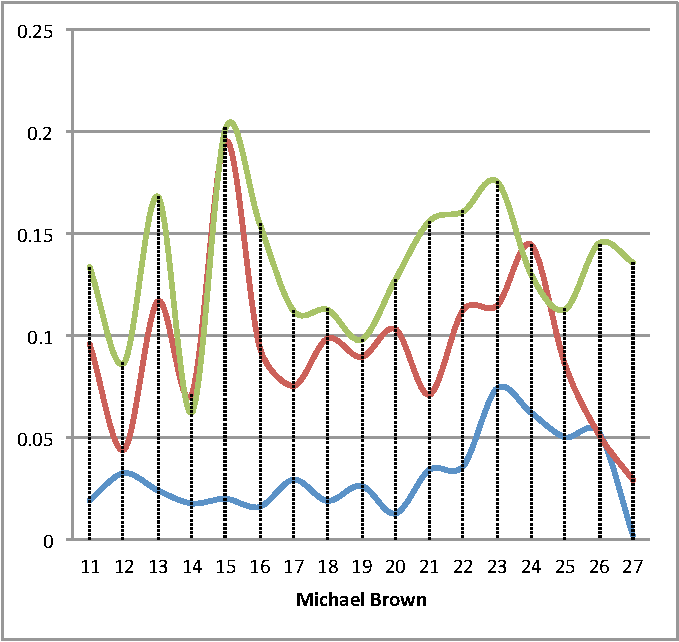
\includegraphics[width=0.22\linewidth]{figures/4_3_Michael_Brown.pdf}
\label{fig:mb}
}
\subfigure[News Report]
{
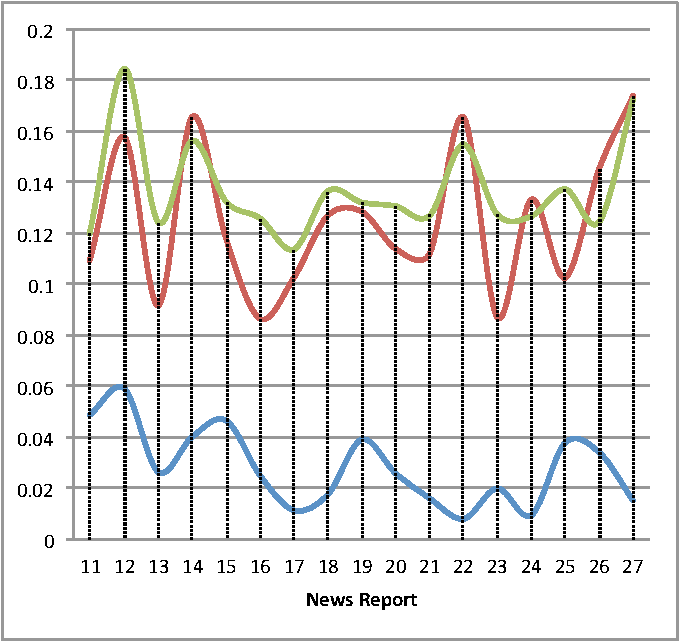
\includegraphics[width=0.22\linewidth]{figures/4_4_News_report.pdf}
\label{fig:news_report}
}
%\subfigure[Racism]
%{
%\includegraphics[width=0.32\linewidth]{figures/4_5_Racism.pdf}
%\label{fig:racism}
%}
\subfigure[Pray]
{
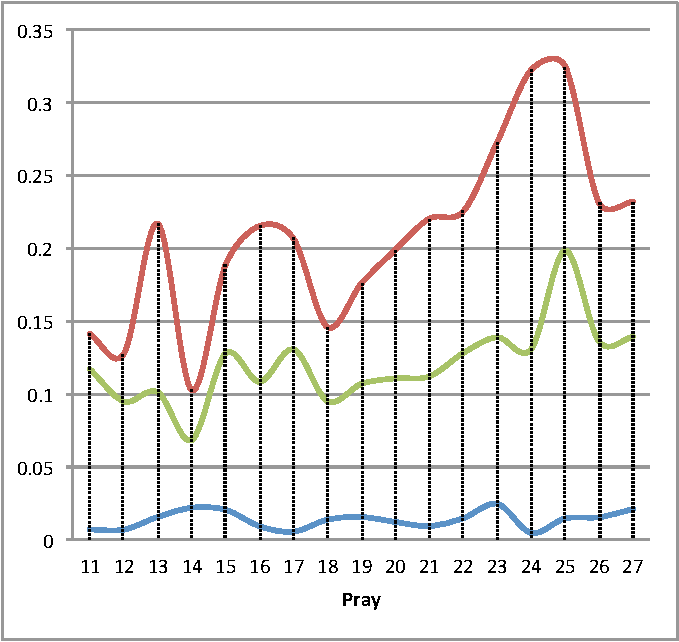
\includegraphics[width=0.22\linewidth]{figures/4_6_Pray.pdf}
\label{fig:pray}
}
\subfigure[Emotion]
{
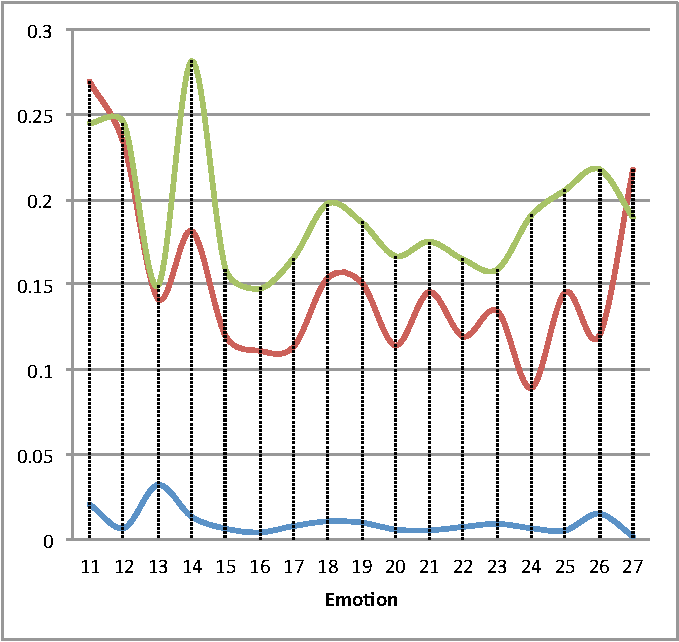
\includegraphics[width=0.22\linewidth]{figures/4_7_Emotion.pdf}
\label{fig:emotion}
}
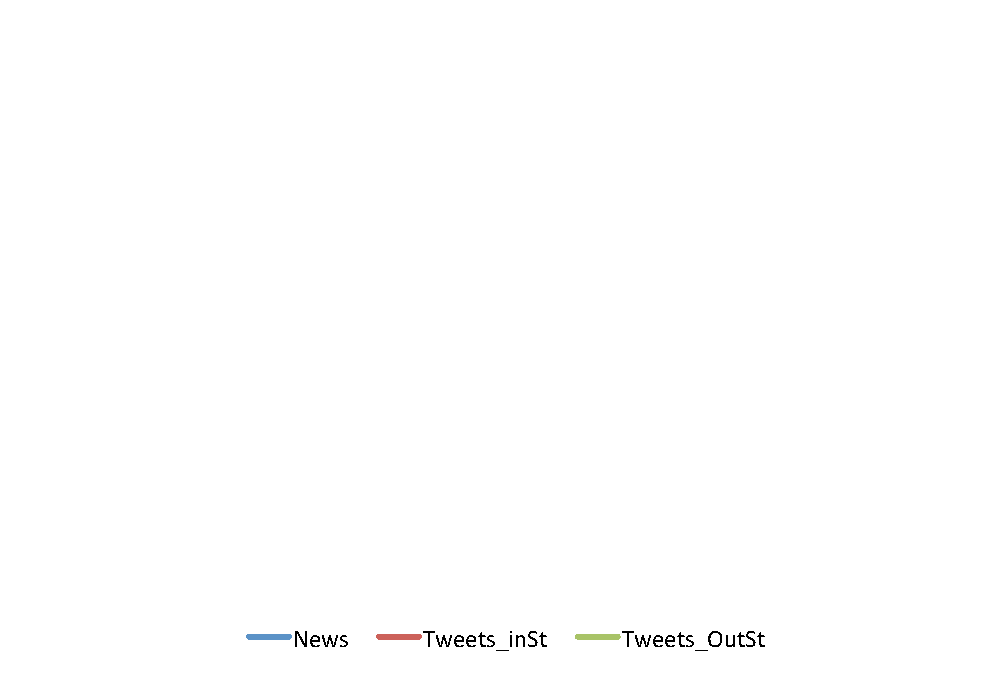
\includegraphics[width=0.5\linewidth]{figures/4_Legend_cut.pdf}
\caption{Topic Dynamic of News and Tweets by \stlda}\label{fig:topics_news_tweets}
\end{figure*}

\subsubsection{Media Influence on the Public}
As Twitter is a self-contained environment, tweets out of \stlouis are also influenced by content in Twitter. So they share similarities with tweets in \stlouis, such as the diversity of topics and similar pattern for topics \pray, \emotion and \newsreport. However analysis of topics also shows that compared to people in \stlouis, their perception of the event relies more on outside source of information rather than self experience, thus they are subjected to be influenced by media more.

Difference between tweets in and out of \stlouis indicates the possible influence from media to the public. Out of \stlouis, the \emotion tweets take the majority on August 12th and 14th, on one day when main media topic is \shootincident, and another day when media increasingly talk about \obamatalk. The rapid growth of \emotion suggests either a long term effect of \shootincident or a quick force of \obamatalk. The two topics are influential, however there is no more fine-grained analysis of what the emotions are, e.g. positive and negative emotions.

\racism is a major topic for tweets out of \stlouis and has an increasing trend, which is consistent with the increasing trend of news talking about \raceandcommunity. The agenda setting of media has actual influence on the public.

In the topic \newsreport, top words such as \emph{news}, \emph{watch}, \emph{live}, \emph{report}, \emph{coverage} and \emph{rt} indicate that the topic is mainly about description or citation of information from news or TV. It is an direct evidence of media influence on tweets. An increase of \newsreport topic tweets means more public attention to news. Interestingly, tweets in and out of \stlouis have similar topic dynamics for \newsreport, meaning that news have similar impact to people both in and out of \stlouis. However, to figure out why the peaks and what news attract public attention, we need more detailed analysis to the reference of news by tweets.

It is also worth noting that proportion of each topic changes more slightly compared to tweets in \stlouis. Although tweets of certain topic may increase in some time, the proportion of tweets in each topic keeps relatively steady. It is possible that people out of \stlouis have different sources of information like news and social media, so their focus is more dispersed under the influence of different information.

\subsubsection{Media Reflection of Public Voices}
In major topics of news, discussion of racism may reflect public concerns, as topic \racism takes an important part of both tweets in and out of \stlouis. It is more likely to be interaction between media and the public with influence in both direction.

Of the minor topics of news, topic \pray and \emotion take a very small part (less than 5\%). It is reasonable that tweets are more subjective and contain more words about feelings, emotions and prays, while news is more serious and objective, avoiding emotional leading. However, even when there is an explosion of \emotion in tweets, or there are increasing tweets talking about \pray, there is no corresponding burst of news topic, which means such emotional change of the public is not reflected in news, or maybe news reacts to the emotions with other topics. However the relation is even harder to detect, because we don't know which news topics are in react to public emotions.
The topic \michaelbrown can be seen as a peak in news followed by increasing tweets of such topic. Then from August 19th increasing tweets in \stlouis start to talk about \michaelbrown again followed by a lag increase pattern of tweets out of \stlouis and news. Except for the funeral of Brown, there are no special events tend to be related to such change. It is possible that when the public pay more and more attention to Michael Brown and the media capture this change and reflect it in news.

In summary, evidence shows the influence of news on tweets, while media reflection of public voices is rare. The existence of \newsreport topic in tweets directly shows the information flow from news to tweets. Comparatively there is no specific topic related to tweets in news. Change of \racism in tweets out of \stlouis may reflect the results of agenda-setting by media. While \emotion change is a possible result by media topics. Because of the media influence, except the main topic \racism, focus of the public is dispersed, while there are different focuses from \emotion, \racism to \protest and \pray along with time for tweets in \stlouis. However, although under the influence of media, tweets do not simply repeat topics of news. Only a small amount of tweets talk about \obamatalk, even though news have steady coverage of \obamatalk during the events. There is no direct evidence showing that news have reflected the opinion changes in tweets. It is possible that news react to tweets topics with other topics, such as the discussion of \raceandcommunity.


\section{Conclusions}
\label{sec:conclu}

To examine interactions between news and media, we propose a new topic model \stlda to bring news and tweets under a unified topic frame, so that topics of news and tweets are comparable. Meanwhile, \stlda shows advantage in processing documents of different lengths, by assigning multiple topics to news and only one topic to each tweet. It avoids representation of noisy topics in tweets, which is usually the case in conventional LDA on tweets.

To large extent, the results support the theory of cascade model~\cite{entman1993framing} from the perspective of the role media play. News have certain topics to cover. Specifically, a certain space of news is occupied by report of the government reaction. The change of major topics is not directly related with corresponding topics in tweets. Even in minor topics, the evidence of news coverage of tweets topics is rare.

However there is evidence of media influence on tweets, thus the existence of \newsreport topic in tweets. Meanwhile tweets out of \stlouis tend to be more influenced by news, so the difference between tweets in and out of \stlouis shows how media influence is. We find major topic \racism is consistent with increasing discussion of race in news. And there are relatively smaller changes of proportion of topics in tweets out of \stlouis, which could be influenced by diverse sources, such as social media, TV and news. The emergence of social media brings diverse opinions to the public. Although under the influence of news media, the public do not show similar focus as the main voice from media. Rather, they share similar emotions and focuses with people in \stlouis who experience and witness what happens. Social media enhances communication between the public and diversifies perspectives of events.


%\section*{Acknowledgement}

The authors would like to thank Prof. Philip Resnik and fellows in LING848 for useful advice.

\bibliographystyle{style/aaai}
\bibliography{bib/journal-full,bib/ref}

%\begin{appendix}

\section{Derivation of ST-LDA Gibbs Sampling Equation}
\label{sec:derivation}

The probability of documents over topics are computed as

\begin{eqnarray}
&&\prob{\bm{z}}{\alpha} \notag \\
&\propto& \int \prob{\bm{z}}{\bm{\theta}} \prob{\bm{\theta}}{\alpha} \mathrm{d}\bm{\theta}\\
&\propto& \int \left( \prod_{k=1}^{K} \theta_k^{N_k} \right) \left( \frac {1} {\Delta(\alpha)} \prod_{k=1}^{K} \theta_k^{\alpha-1} \right) \mathrm{d}\bm{\theta}\\
&\propto& \int \frac{1}{\Delta(\alpha)} \prod_{k=1}^{K} \theta_k^{N_k+\alpha-1} \mathrm{d}\bm{\theta}\\
&\propto& \frac{\Delta(\bm{N}+\alpha)}{\Delta(\alpha)},
\end{eqnarray}
where $\Delta(\cdot)$ is defined as

\begin{equation}
\Delta(\bm{x}) = \frac {\prod_{k=1}^{K} \Gamma(x_k)} {\Gamma(\sum_{k=1}^{K} x_k)}.
\end{equation}

The probability of words over topics are computed as

\begin{eqnarray}
&&\prob {\bm{w}} {\bm{z}, \beta} \notag \\
&\propto& \int \prob {\bm{w}} {\bm{z}, \bm{\phi}} \prob {\bm{\phi}} {\beta} \mathrm{d} \bm{\phi}\\
&\propto&\int \left( \prod_{k=1}^{K} \prod_{v=1}^{V} \phi_{k,v}^{N_{k,v}} \right) \left( \prod_{k=1}^{K} \frac {1} {\Delta(\beta)} \prod_{v=1}^{V} \phi_{k,v}^{\beta-1} \right) \mathrm{d} \bm{\phi}\\
&\propto&\int \prod_{k=1}^{K} \frac {1} {\Delta(\beta)} \prod_{v=1}^{V} \phi_{k,v}^{N_{k,v}+\beta-1} \mathrm{d} \bm{\phi}\\
&\propto&\prod_{k=1}^{K} \frac {\Delta(\bm{N_k}+\beta)} {\Delta(\beta)}.
\end{eqnarray}

Therefore, the joint probability of words and topic assignments is 

\begin{equation}
\prob {\bm{w}, \bm{z}} {\alpha, \beta} = \frac {\Delta(\bm{N}+\alpha)} {\Delta(\alpha)} \prod_{k=1}^{K} \frac {\Delta(\bm{N_k}+\beta)} {\Delta(\beta)}.
\end{equation}

Finally the Gibbs sampling equation is derived as

\begin{eqnarray}
&&\prob {z_{d}=k} {\bm{z_{-d}},\bm{w_d}} \notag \\
&\propto& \frac {\Delta(\bm{N}+\alpha)} {\Delta(\bm{N^{-d}}+\alpha)} \frac {\Delta(\bm{N_k}+\beta)} {\Delta(\bm{N_k^{-d}}+\beta)}\\
&\propto& \frac {\Gamma(N_k+\alpha)} {\Gamma(N_k^{-d}+\alpha)} \frac {\Gamma(N_{\cdot}^{-d}+K\alpha)} {\Gamma(N_{\cdot}+K\alpha)} \notag \\
&&\frac {\Gamma(N_{k,\cdot}^{-d}+V\beta)} {\Gamma(N_{k,\cdot}+V\beta)} \prod_{v=1}^{V} \frac {\Gamma(N_{k,v}+\beta)} {\Gamma(N_{k,v}^{-d}+\beta)}\\
&\propto& \frac {N_{k}^{-d}+\alpha} {N_{\cdot}^{-d}+K\alpha} \frac {\prod\limits_{v=1}^{V} \prod\limits_{i=0}^{N_{d,v}-1} (N_{k,v}^{-d}+\beta+i)} {\prod_{i=0}^{N_{d,\cdot}-1} (N_{k,\cdot}^{-d}+V\beta+i)}\\
&\propto& \left( N_{k}^{-d}+\alpha \right) \frac {\prod\limits_{v=1}^{V} \prod\limits_{i=0}^{N_{d,v}-1} (N_{k,v}^{-d}+\beta+i)} {\prod_{i=0}^{N_{d,\cdot}-1} (N_{k,\cdot}^{-d}+V\beta+i)}.
\end{eqnarray}

\end{appendix}

\end{document}
